\subsection{Overview}
As stated above, each subsystem has to accomplish its own goal. In particular, we can see AutomatedSOS and Track4Run as simple  applications for smart-devices, while Data4Help is a service provider that should implement a more complex, scalability-oriented architecture.

The figure below gives a general overview of a possible implementation of the system.

\FloatBarrier

\begin{figure}[!h]
	\centering
	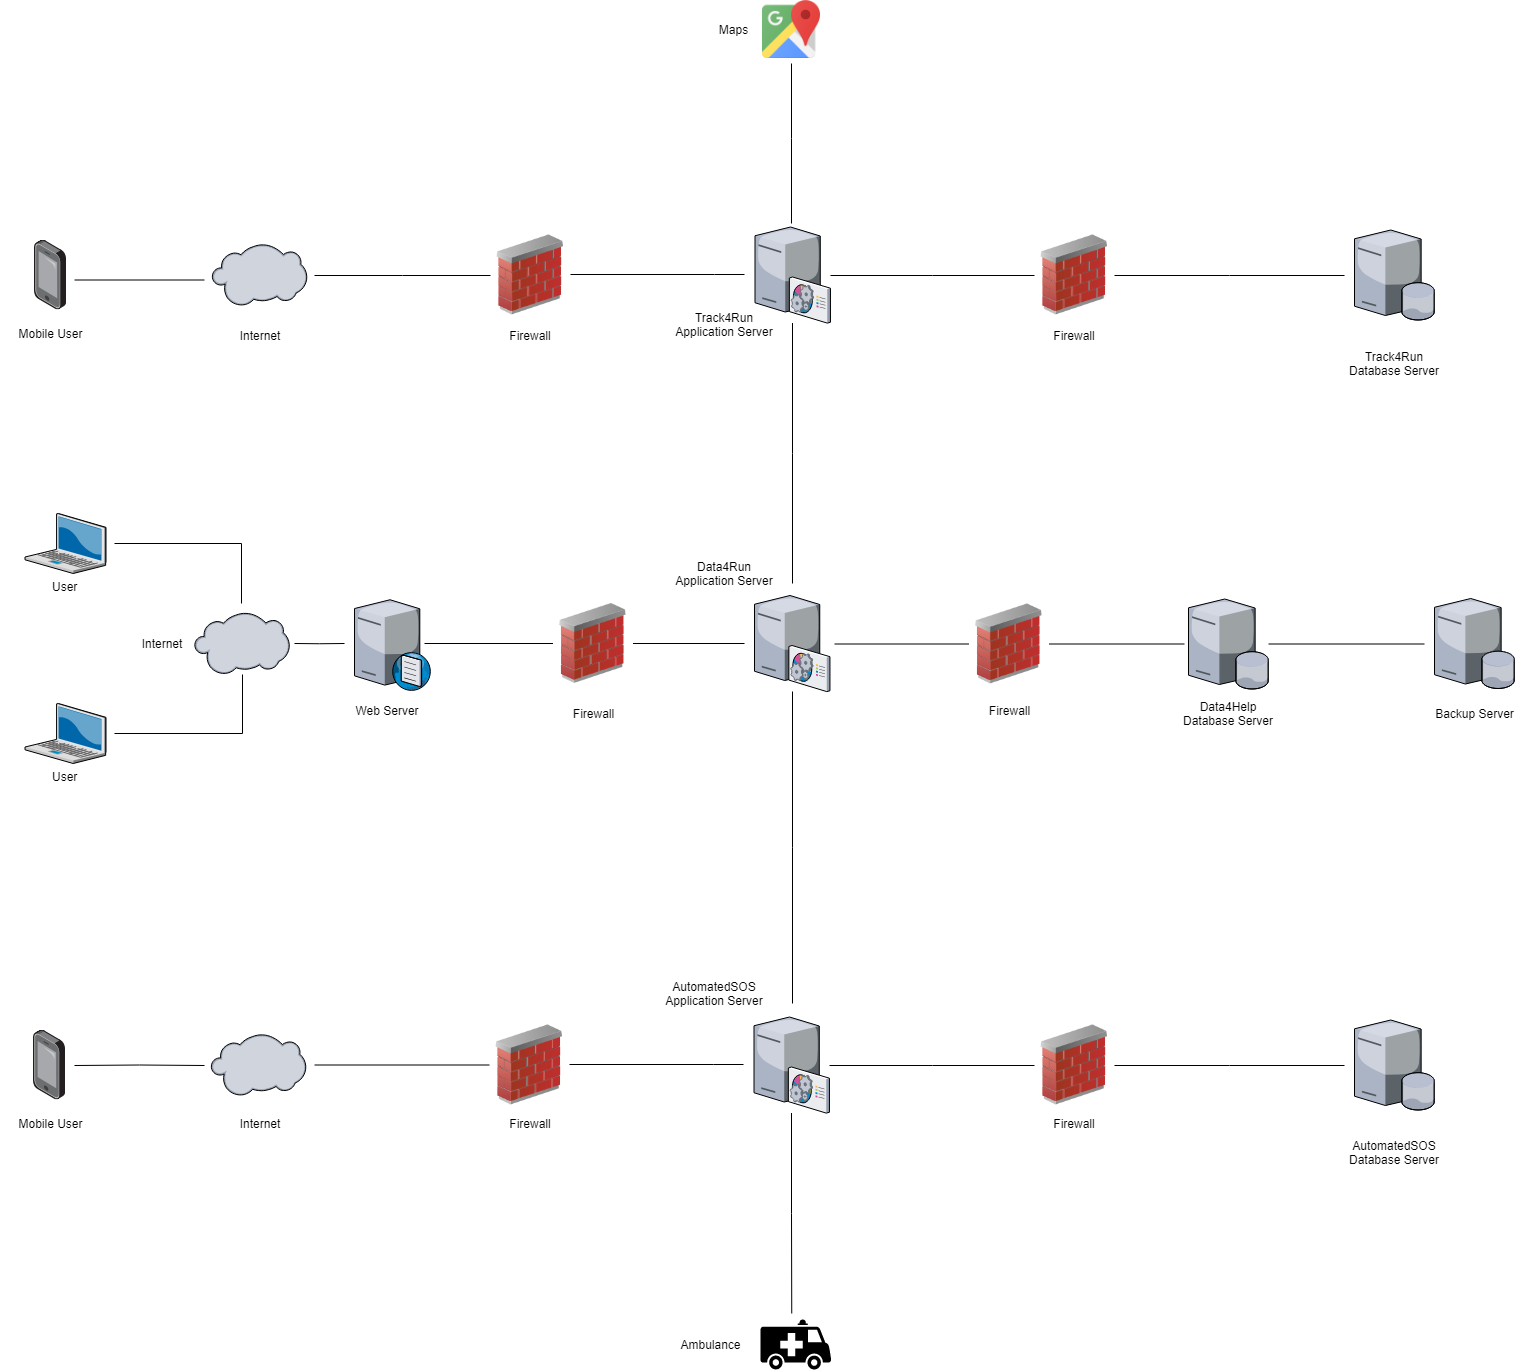
\includegraphics[width=0.9\columnwidth]{physicalArchitectureDiagram.png}
	\caption{General Architecture}
\end{figure}


\FloatBarrier

As displayed in this figure, Data4Help subsystem's services can be accessed by many channels, in particular a web interface for the end users and an API for data-sources and third-party applications.

The data-source devices will provide the system with real-time user data, hence it is predictable that this flow of information will soon grow into a huge number of requests. For this reason, this subsystem has to be designed to quickly accomplish horizontal scaling and maintain high availability even in extreme conditions.
In particular, a Microservice based architecture enforced with Message Queues and scalable databases should be adopted, as will be described in the following sections. Also an API Gateway is used to access all Data4Help interfaces, so to easily manage authentication and load balancing from the very first moment of any request.

AutomatedSOS and Track4Run are instead designed as three-tier applications with a thick client (i.e. smart-phone and smart-watch apps), a lightweight back-end server and a storage module. This design has been chosen because it is completely modular on one hand, since the two application's business logic is separated from Data4Help's one, and guarantees on the other hand a fast and reliable service from the back-end servers, leaving the full responsibility of the presentation part to the mobile application. The separation of presentation and business logic also guarantees the maintainability of the system and good performances on mobile devices, where power consumption and CPU usage can be an issue.

\subsection{High Level Architecture}

From the component point of view, each subsystem can be divided into \textit{back-end} components, which are responsible of carrying out the business logic of the subsystem, and \textit{front-end} components, which provide a presentation layer to end users and SDKs to external developers who want to access the system's services.
Also, some external components are used to provide some of the services offered by the system.

In the following diagram, the main components and interfaces are highlighted, to give a general idea of the design of the system.
It must be noted that in this diagram components and \textit{modules} represent a set of services grouped together, and internal interactions between modules are not shown for sake of simplicity: this description will be done in the following sections.

\FloatBarrier
\begin{figure}[!h]
	\centering
	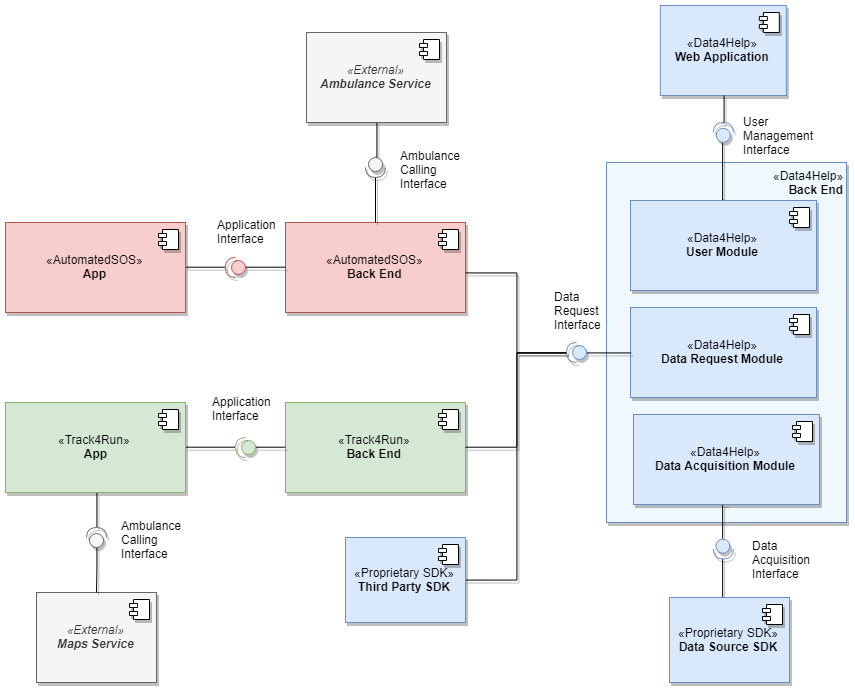
\includegraphics[width=\columnwidth]{ComponentDiagrams-Total.png}
	\caption{High Level Components}
\end{figure}
\FloatBarrier

As can be seen, the Data4Help back-end is composed of four major modules:

\begin{itemize}
	\item \textit{User Management}: provides an interface for managing the user account and configure his data-sources. This interface is exploited by a \textit{Web Application} that can be accessed via web browser.
	\item \textit{Data Acquisition}: provides the interface for collecting data from data-sources. A proprietary \textit{Data Source SDK} can be offered to external developers to integrate the use of this interface into their software and send data from external devices to Data4Help.
	\item \textit{User Management}: enables third parties to make requests on the data received by the subsystem. This interface is used by \textit{Track4Run} and \textit{AutomatedSOS} back-ends, but it can also be accessed by any other third party via the dedicated \textit{Third Party SDK} that is offered to third-party developers.
	\item \textit{Authentication}: enables the system to recognize and authenticate incoming requests and associate them to a specific User, Third Party or Data-Source.
\end{itemize}

The other two back-ends are mainly responsible of exploiting Data4Help's serviced to offer an interface to the user's Application. 

\begin{itemize}
	\item \textit{AutomatedSOS App Interface}: provides the functions to login a user, modify its threshold and monitor its health state.
	\item \textit{Track4Run App Interface}: provides the functions to login a user, create and modify a run, search runs, join a run a watch runners.
\end{itemize}

Finally there are the external services: for AutomatedSOS, an external ambulance calling interface is needed by the back-end to fulfill its goals, while in Track4Run a Maps Service such as \textit{Google Maps} should be accessed directly from the Application to minimize latency and bandwidth occupation in the communication between the client and the server.

Another definition of the services offered by the system can be found in the figure below, which highlights the dependencies between the Data4Help system and its actors and provides a list of the services consumed internally and externally by the system.

\FloatBarrier
\begin{figure}[!h]
	\centering
	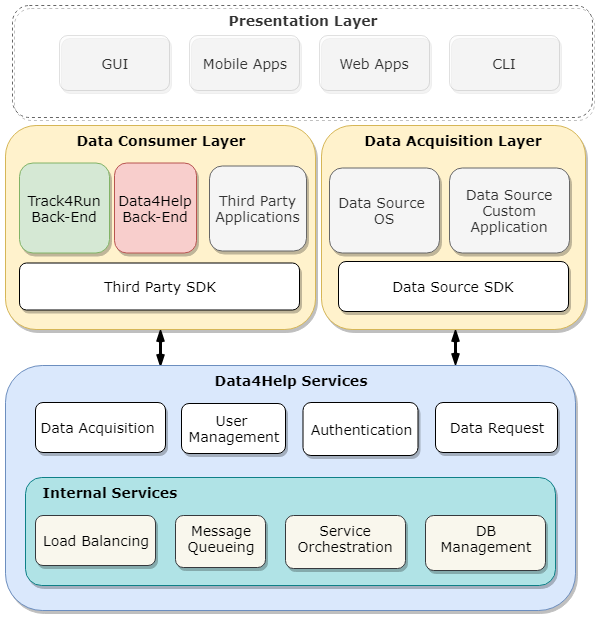
\includegraphics[width=0.8\columnwidth]{ComponentDiagrams-Layers.png}
	\caption{System Layers Architecture}
\end{figure}
\FloatBarrier

The whole system's internal and external services can be divided into five layers:
\begin{itemize}
	\item \textit{D4H Internal Services Layer}: these components are used internally by Data4Help to provide highly available services. They mainly deal with microservices management and will not be discussed in the detailed architecture, since there are many available options on the market such as Docker and Kubernetes for container management, MongoDB for data management, RabbitMQ for message queueing etc...
	
	\item \textit{D4H External Services Layer}: this layer provides the four main functionalities of Data4Help, which have been discussed in the previous part.
	
	\item \textit{Data Acquisition Layer}: this layer is built upon Data4Help Services. It contains the SDK on which external data-source software can rely to send collected data to Data4Help.
	
	\item \textit{Data Consumer Layer}: also this layer is built upon Data4Help Services and contains the SDK that can be used by third parties to make API requests, as well ad the whole AutomatedSOS and Track4Run back-ends, which are in this sense \textit{consumers} of the Data4Help services.
	
	\item \textit{Presentation Layer}: can be built upon the previous layers, in the case of AutomatedSOS and Track4Run, this layer represents the mobile application, which provides a GUI to the end user. Also data-sources and external third-parties can offer a presentation layer to their end-users.
\end{itemize}


\subsection{Component View}


\subsubsection{Data4Help}

Here is a detailed view of the components of the Data4Help subsystem: each service is to be considered as independently deployed and can be replicated in many instances, following the typical microservice cluster architecture. 


\FloatBarrier
\begin{figure}[!h]
	\centering
	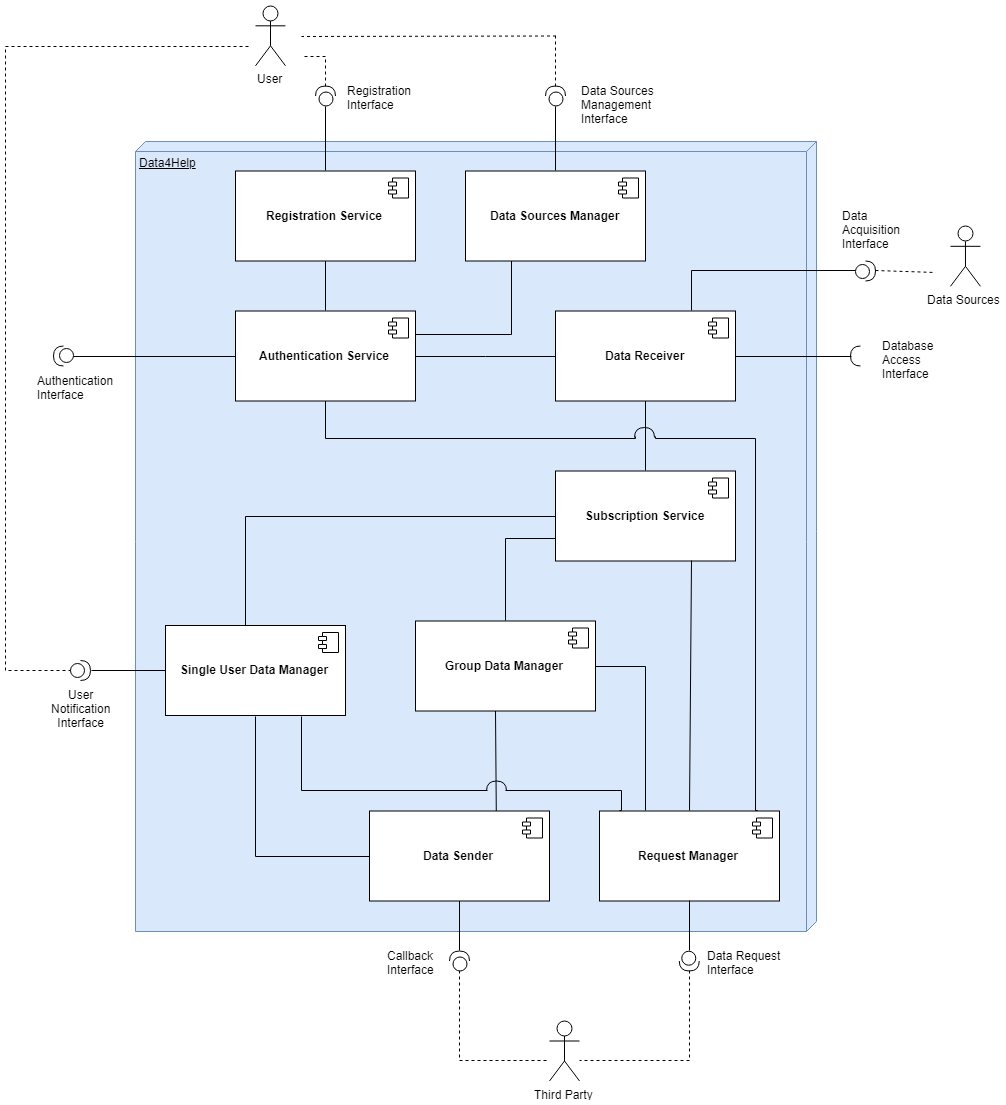
\includegraphics[width=\columnwidth]{ComponentDiagrams-Data4Help.png}
	\caption{Data4Help Components}
\end{figure}

\FloatBarrier

The internal microservices that have been identified are:
\begin{itemize}
	\item \textbf{API Gateway}: This is the single entrypoint through which all other services can be accessed. For more information see \textit{API Gateway Pattern} in \textit{Section 2.7}. In this diagram, other components are also represented in the API Gateway:
	\begin{itemize}
		\item \textit{Load Balancer:} realizes the balancing between different instances of the same services, deciding where to redirect each request.
		\item \textit{Service Registry:} keeps track of all the deployed services instances.
		\item \textit{Service Orchestrator:} is responsible of managing the deployment of new service and manage the failure of existing ones..
		\item \textit{Message Broker:} enables messaging between services.
	\end{itemize}
	Please note that the interaction between these components and the rest of the system is not represented, for the sake of simplicity. All these services are part of the internal services layer as already mentioned, and are considered to be something already present during the development of this system.
	\item \textbf{Authentication Service}: this service is in charge of producing tokens when new users register and verifying incoming tokens when requests are made to the API Gateway.
	\item \textbf{User Service}: this service provides an interface for the Web Application. The main functions of this service are Account Management functions, such as password changing, name setting etc., and functions related to the management of the preferred data-source for each tracked parameter.
	\item \textbf{Receiver}: this service is responsible of managing a new incoming data-source packet, verifying the user preferences for that data-source and eventually saving the packet on the DB. It is also responsible of notifying the subscription service with the ID of the received parameter, so that the appropriate third parties can be notified of the new data.
	\item \textbf{Request Manager}: this component is responsible of receiving and parsing the data requests coming from third-parties.
	
	In case of one-shot requests, a user notification service will be called to ask the user's permission, and then the sender service will be invoked to send the actual response.
	If the request is instead a subscription request, this will be saved in the DB after the user's approval.
	
	Group requests don't need user approval, but they need to be filtered through the anonymization service.
	\item \textbf{Sender}: this service is in charge of consuming the sender queue, build the request for each response and send the response to the corresponding callback interface.
	\item \textbf{Subscription Service}: this component is in charge of consuming the notifications received by the receive service(s) and control if the new data fits into to a single user or group data subscription. In this case, the corresponding response will be queued in the sender queue.
	\item \textbf{Anonymization Service}: this service simply tells if a given group request ca be properly anonymized. It can be accessed by a synchronous protocol.
\end{itemize}

This subsystem shall also use messaging between microservices where asyncronous communication is possible, while all other components shall use synchronous protocols, such as RESTful APIs.

\subsubsection{AutomatedSOS}

\FloatBarrier
\begin{figure}[!h]
	\centering
	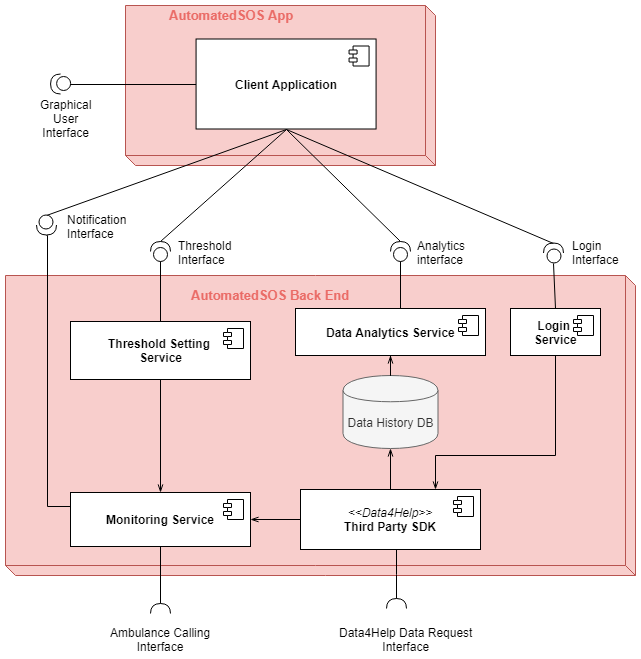
\includegraphics[width=\columnwidth]{ComponentDiagrams-AutoSOS.png}
	\caption{AutomatedSOS Components}
\end{figure}
\FloatBarrier

\begin{itemize}
	\item \textbf{Client Application:} application on user's device responsible of providing a graphical interface to the user and of interacting with the back end  services of AutomatedSOS.
	\item \textbf{Threshold Setting Service:} gives to the user the possibility to change the default threshold values of his tracked parameters and save them in the dedicated database. 
	\item \textbf{Data Analytics Service:} allows the user to check the aggregated statistics about the data collected until then with a given granularity. 
	\item \textbf{Login Service:} responsible of authenticating the user by using his Data4Help credentials using the SDK services provided by the Third Party SDK component.
	\item \textbf{Monitoring Service:} is responsible of monitoring the data coming from Data4Help and, whenever a threshold is exceeded, interacting with the external Ambulance Calling Interface which in turn will communicate to the ambulances the location of the user in danger.
	\item \textbf{Third Party SDK:} communicates with Data4Help by using his Authentication and Data Request interfaces.
\end{itemize}


\subsubsection{Track4Run}

\FloatBarrier
\begin{figure}[!h]
	\centering
	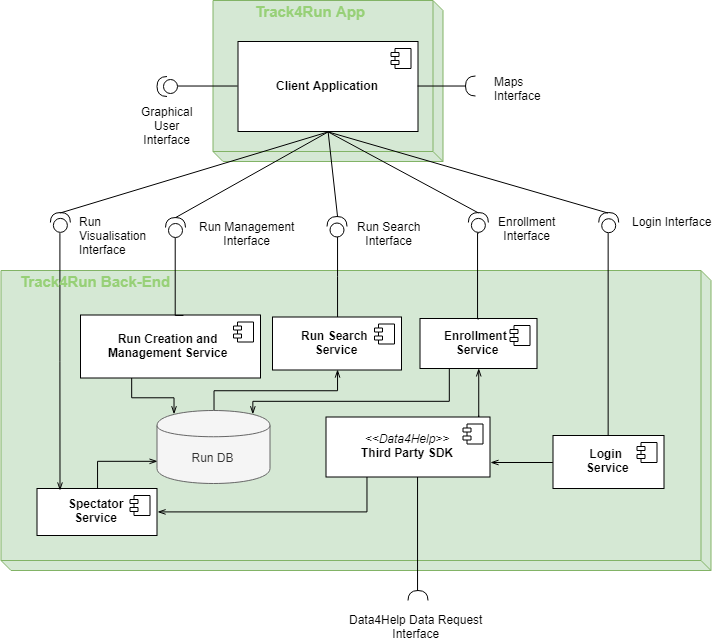
\includegraphics[width=\columnwidth]{ComponentDiagrams-Track4Run.png}
	\caption{Track4Run Components}
\end{figure}
\FloatBarrier

\begin{itemize}
	\item \textbf{Client Application:} application that runs on user's device responsible of providing a graphical interface to the user and of interacting with the back end services of Track4Run. It also interacts with an external Maps Interface in order to retrieve the maps that will be used by the application.
	\item \textbf{Run Creation and Management Service:} gives the user the possibility to create, edit and delete a run event by interacting with the Run database.
	\item \textbf{Run Search Service:} gives the user the possibility to browse all the created run events stored in the Run database.
	\item \textbf{Spectator Service:} is responsible of retrieving runners position during the run and then forwarding it to the Client Application which in turn will display the positions of the runners on a map.
	\item \textbf{Enrollment Service:} allows the user to enroll in a created run event. In this way he will be added to the list of participants.
	\item \textbf{Third Party SDK:} communicates with Data4Help by using his Authentication and Data Request interfaces.
	\item \textbf{Login Service:} responsible of authenticating the user by using his Data4Help credentials using the SDK services provided by the Third Party SDK component.
\end{itemize}

\subsubsection{Entity-Relationship Diagram}
The following diagram provides a graphical representation of the data entities of the system. In the diagrams, different colours represent the three different subsystems.

\FloatBarrier
\begin{figure}[!h]
	\centering
	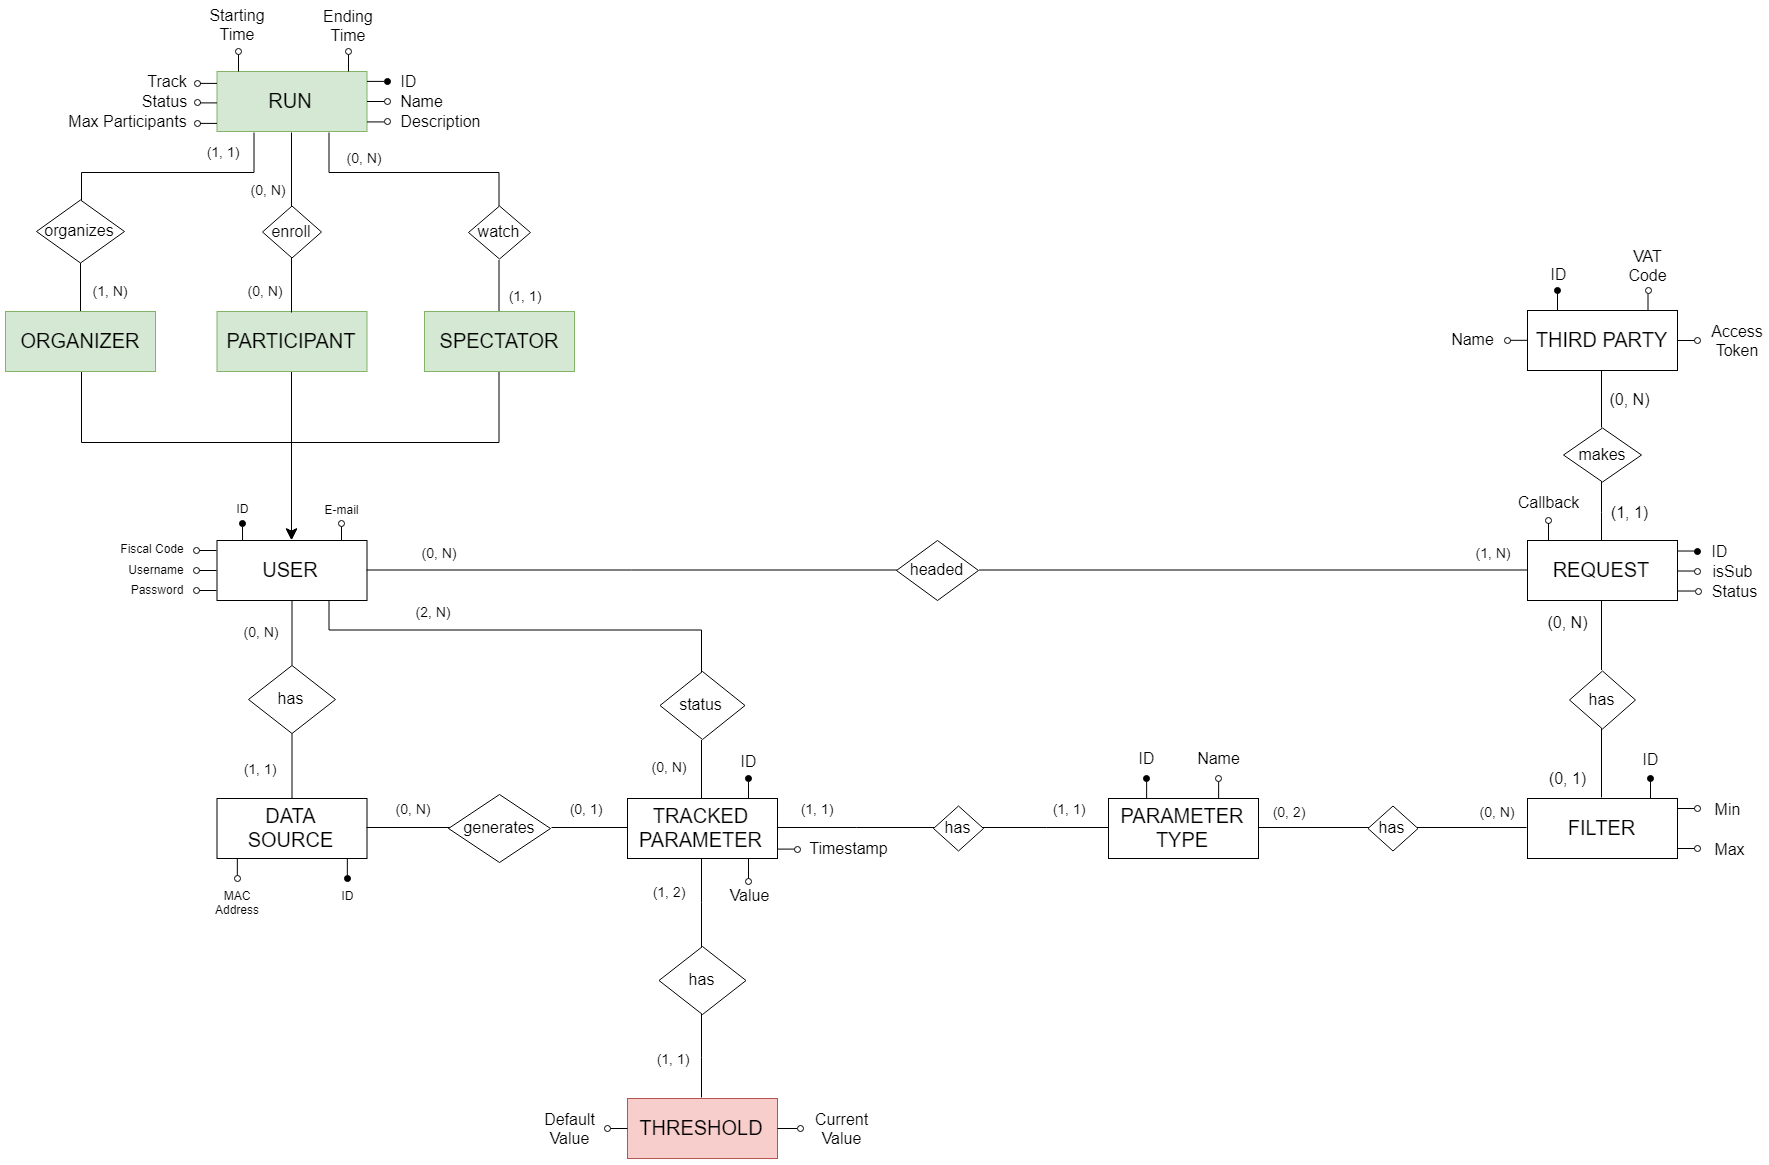
\includegraphics[width=\columnwidth]{ER.png}
	\caption{Entity-Relationship Diagram}
\end{figure}
\FloatBarrier


\subsection{Deployment View}

The deployment for the three subsystems reflect the architecture that has been described in the previous sections. In particular, the AutomatedSOS and Track4Run deployment will follow a simple application-style pattern, with a Node.js back-end that can be easily built and a standard SQL DB.

Data4Help on the onther hand follows the microservices pattern, in particular the API Gateway and Service Discovery patterns: a Gateway API, deployed on a dedicated machine, will filter all the incoming request and forward them to the single services. Every back-end service is instead deployed in a container, that can be located in a physical or virtual machine, and new instances of a service can be deployed when needed. On the side of this microservice cluster, entities such as a container orchestrator, a load balancer, a service registry and a message broker are needed to properly manage the cluster. These have to be deployed in a dedicated and reliable machine of the internal network.

\FloatBarrier
\begin{figure}[!h]
	\centering
	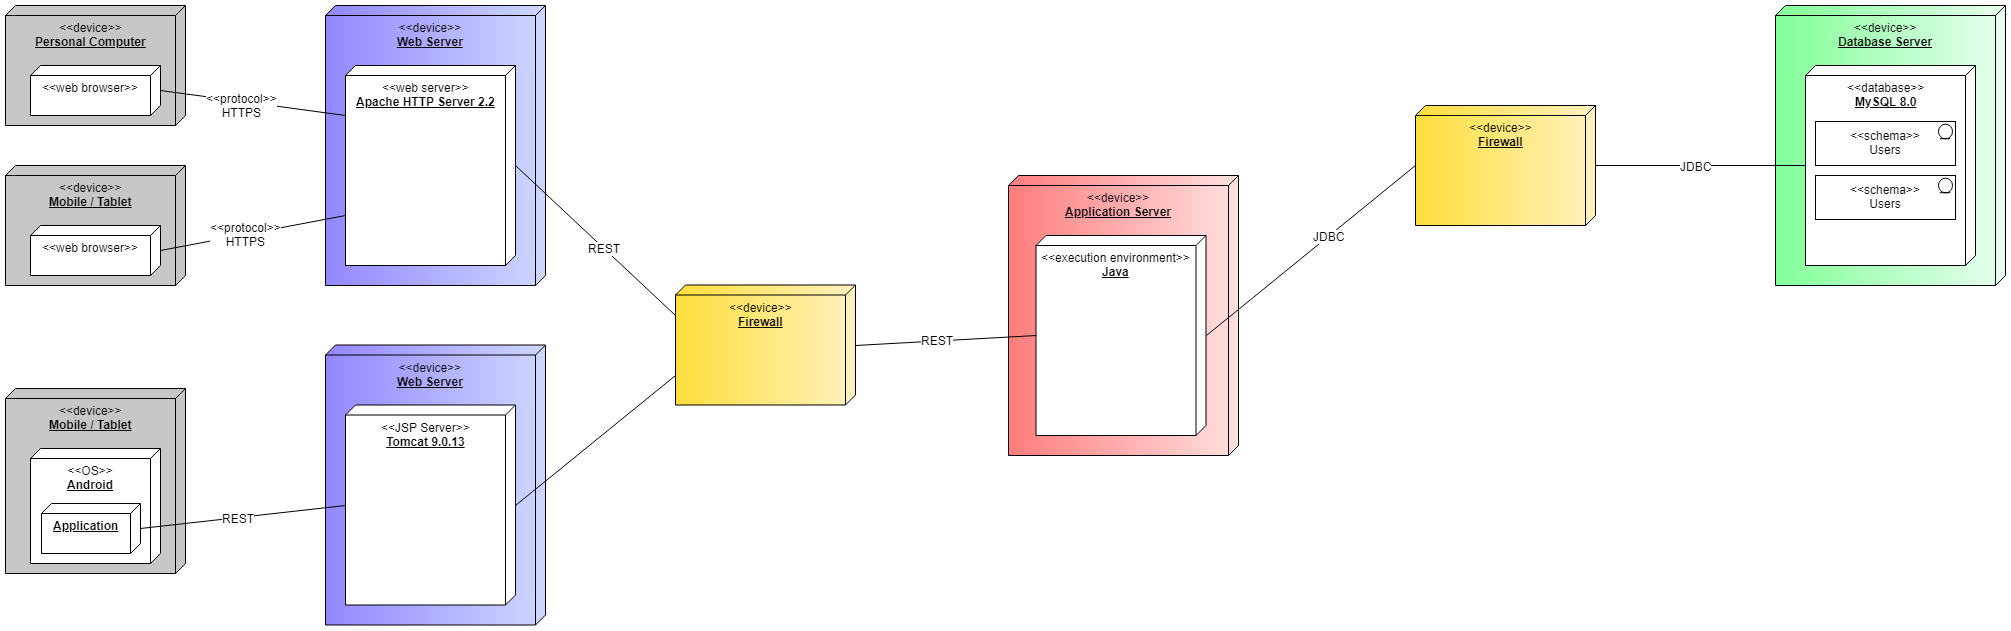
\includegraphics[angle=90, height=0.9\textheight]{deploymentDiagram.png}
	\caption{System Deployment Diagram}
\end{figure}
\FloatBarrier

\subsection{Runtime View}
Many sequence diagrams which show the interaction between the users and the system are already present in the RASD. However, some of the internal details of the runtime phase of our application will be given below.

\begin{itemize}
	\item \textbf{auth}
\end{itemize}
	
- new data
- sub
- one-shot
- group

\subsection{Component Interfaces}

\FloatBarrier
\begin{figure}[!h]
	\centering
	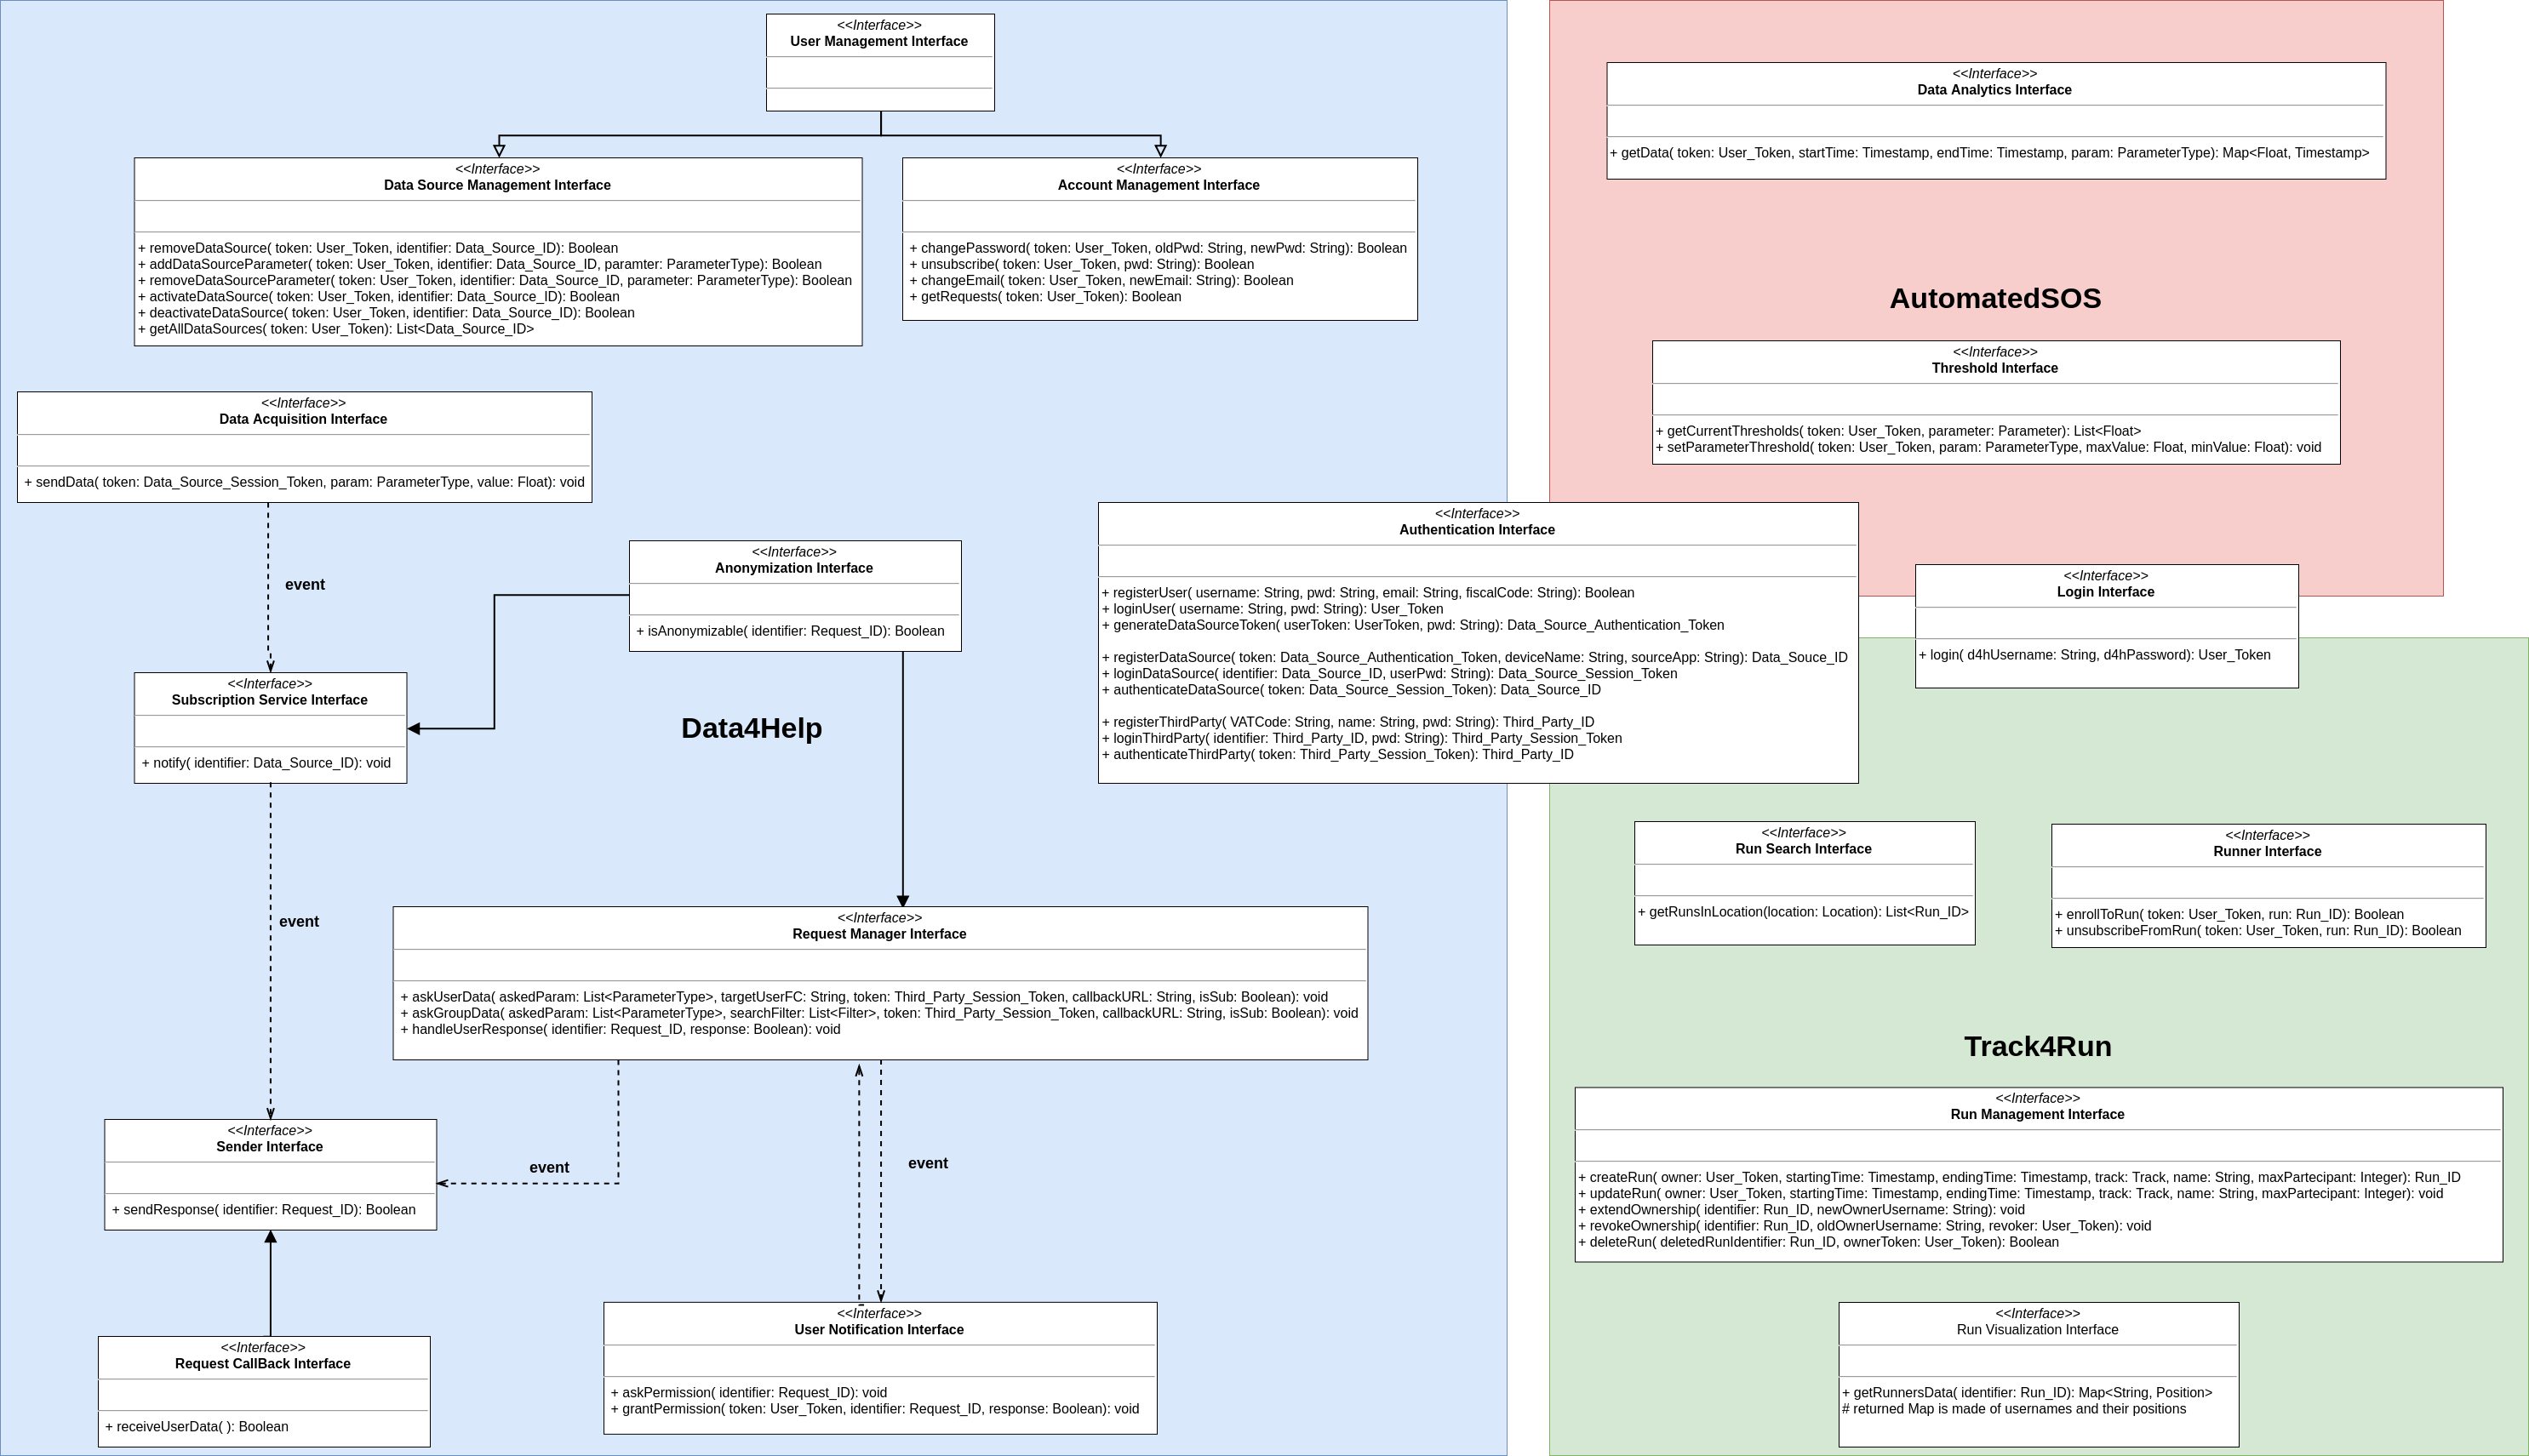
\includegraphics[width=\linewidth]{ComponentInterfaceDiagram.png}
	\caption{Component Interface Diagram}
\end{figure}
\FloatBarrier

\subsection{Selected Architectural Styles and Patterns}
\begin{itemize}
	\item \textbf{Loose Coupling}: the first principle we followed in the design of the whole product is loose coupling, which means that we tried to minimize the dependencies between components of a subsystem and between the three subsystems as well. This means that each subsystem can be developed, deployed and maintained separately, which gives to the system a good flexibility for future development.
	
	\item \textbf{Stateless Components}: since one of our major concerns is the reliability of our system and how good it recovers from situations of partial unavailability, our components are designed to be stateless. This means that each component reads and writes on a DataBase at every step of its work, so that if one of the services is temporarily down, its state can be easily recovered from the DB.
	
	\item \textbf{MVC}: For AutomatedSOS and Track4Run subsystems, we decided to adopt a standard \textit{Model-View-Controller} monolithic architecture. This gives the possibility to the developers of this subsystems to use well-known commercial solutions to implement this applications.
	
	\item \textbf{Client-Server Pattern}: The classical division of the MVC pattern between Model and View is reinforced by using the client-server pattern, in which there is a client which asks for resource and a server that must provided these resources. For AutomatedSOS and Track4Run the client is a \textit{Thick-Client} which takes care of the whole presentation part, whereas in the Data4Help subsystem we have a \textit{thin-client} application for the users, which is their browser.
	
	\item \textbf{Microservice Architecture Pattern}: For Data4Help instead we decided to implement a microservice architecture patter. The idea behind a microservice-based architecture is to apply the \textit{SOA} pattern (\textit{Service Oriented Architecture}) inside a big project, breaking it down in small pieces that act independently, communicate asynchronously and can be deployed in any fashion and number. This pattern is used in Data4Help because the achievement of high availability and scalability can be easily reached by decoupling the single functions of the system and deploying them independently in large numbers.
	
	In particular, for this microservice design we decided to adopt the following principles:
	\begin{itemize}
		\item \textit{API Gateway Pattern}: A single entrypoint is provided for external access to the services. This gateway will then redirect the incoming calls to the single service. This gives us the possibilities to  unify the management of request authentication, load balancing and eventually performance testing. Please note that the gateway too can be scaled by adding another gateway that have the same service registry in common.
		
		\item \textit{Server Side Discovery}: This method is a way of keeping track of which are the services available on the system an where their instances can be found. It uses a \textit{Service Registry} at a known location where new services register themselves when deployed, so that the Gateway/Load Balancer can read the register to know where to redirect requests.
		
		\item \textit{Asynchronous Queueing}: This pattern is used together with the \textit{Event Driven Architecture} pattern to achieve asynchronous and non-blocking communication between services. In our case, we implement asynchronous queueing when using message queues for sharing information and notifications between services. In this way, when service A has to call service B, it only has to send a message and then it can continue with his job, even if the other service is temporarily unavailable.
		
		\item \textbf{Access Tokens}: The API Gateway authenticates the request and passes an access token that securely identifies the requestor in each request to the services. A service can include the access token in requests it makes to other services.
	\end{itemize}

	\item \textbf{RESTful API}: When asynchronous communication is not possible or desirable, for example during external calls to the system's services, a REST architecture is use to build RESTful APIs that can be accessed by software written in any language. This is another way in which we decouple the functions of our system.
\end{itemize}


\subsection{Other Design Decisions}
While taking design decisions, some implementation-level solutions have been explored to better understand the possible problems during the implementation of the system.
In particular, these are some technologies that have been taken in account.

\begin{itemize}
	\item  \textit{NoSQL Databases}: One of the key features of these kind of databases is scalability, and apparently they are very integrated in many frameworks used for developing microservices, so these kind of databases should be taken in account.
	\item  \textit{JWT}: JSON Access Token is one of the standards for authentication. It is lightweight, cross-platform and easy to use. Alternatively, a possible solution to authentication could be using \textit{Oauth2} servers.
	\item  \textit{Containers}: containers are used a lot in microservices deployment, and should be considered for the implementation of the Data4Help subsystem: they have some security drawbacks with respect to Virtual-Machines or other cloud-based solutions, but surely are a fast and reliable way to manage many instances in a microservice cluster.
	\item  \textit{Real-Time Performance Analyzer}: some services, like \textit{Prometheus} for example, enable the analysis of a container cluster to monitor performance. This tools an be easily used to dynamically scale our application if more or less computational power is needed over time.
\end{itemize}